\chapter{Resultados}
\label{cap:resultados}

Neste capítulo serão apresentados e analisados todos os resultados obtidos do treinamento do \textit{Proximal Policy Optimization} (PPO) para jogar os jogos disponibilizados pela ferramenta GVGAI\_GYM, \textit{Aliens}, \textit{Boulder Dash} e \textit{Missile Command}. Os jogos selecionados variam em termos de recompensas que eles oferecem, e as recompensas disponíveis possuem um grande impacto no sucesso do aprendizado por reforço. Para cada um dos jogos, foi modificado o tamanho do conjunto de treinamento, ou seja, a quantidade de fases disponíveis para treinamento, sendo divididos em conjuntos com um nível de treinamento (PPO1), dois níveis de treinamento (PPO2) e três níveis de treinamento (PPO3). 

Cada fase de um jogo difere em sua dificuldade, definindo o quão desafiante é o jogo. O nível de dificuldade varia na adição ou remoção de eventos desafiadores ou obstáculos para alcançar o objetivo final. A medida que um jogador avança nas fases disponíveis, ele esbarra em desafios cada vez mais complexos, exigindo mais planejamento estratégico e reações rápidas para ser capaz de lidar com as adversidades.

Durante o treinamento do agente uma política é selecionada para interagir com o ambiente em um número fixo de etapas, com o objetivo de coletar um conjunto de experiências. Essas experiências são então utilizadas para atualizar o modelo. Para cada lote de experiências é calculado uma média das recompensas totais dos últimos dez episódios concluídos. A cada dez atualizações do modelo o agente é submetido a uma avaliação de desempenho nos ambientes de testes. A Figura \ref{fig:resultados} contém as informações suavizadas\footnote{O filtro de Savitzky-Golay pela biblioteca Scipy foi utilizado como uma janela de tamanho 53 e ordem polinomial 3.} de média das recompensa obtidas pelo agente durante o treinamento (cores mais escuras) e uma média das recompensas de dez episódios da fase de avaliação (cores mais claras). 

A medida que o número de interações com o ambiente aumenta é esperado que as recompensas durante o treinamento também aumentem: cada atualização deve levar a políticas que maximizem cada vez mais a recompensa obtida. Se o treinamento chegar a tal ponto em que a cada atualização não é observado uma mudança significativa dos valores de retorno, como visto na Figura \ref{subfig:missilecommand-r} para o PPO1,então diz-se que foi atingido um máximo local do problema de otimização da política. 

\begin{table}[H]
\centering
 \begin{tabular}{||c c c c c c c ||} 
 \hline
 Jogos & Agente Aleatório & PPO 1 & PPO 2 & PPO 3 & DQN & A2C\\ [0.5ex] 
 \hline\hline
 Aliens & 38 & 62.7 & 62.7 & 63.5 & 75 & \textbf{77}\\ [1ex] 
 \hline
 Boulder Dash &  1.69 & 19.8 & 19.8 & \textbf{20} & 2.5 & 15.5\\ [1ex] 
 \hline
 Missile Command & -1.46 & 5 & \textbf{11.6} & 10.3 & 5 & 5\\ [1ex] 
 \hline
\end{tabular}
\caption{Comparação das recompensas obtidas para cada jogo.}
\label{tab:allgames}
\end{table}

Na Tabela \ref{tab:allgames} é possível comparar os melhores resultados de treinamento de cada jogo com os melhores resultados dos algoritmos de aprendizado por reforço \textit{Deep Q-Network} (DQN) \cite{mnih13} e \textit{Advantage Actor Critic} (A2C) \cite{openaibaselines} obtidos de Torrado et.tal. \cite{torrado18}, e de um agente com política aleatória. Em ambos \textit{Boulder Dash} e \textit{Missile Command} o algoritmo PPO se sobressaiu aos demais, obtendo pior desempenho apenas no jogo \textit{Aliens}.

Apesar de não ter ultrapassado os outros algoritmos de aprendizado por reforço (Tabela \ref{tab:allgames}), o agente no jogo \textit{Aliens} conseguiu aprender a jogar o jogo razoavelmente bem no conjunto de treinamento. Todos os personagens não-jogáveis e projéteis deste jogo se comportam de maneira determinística e o jogo pode ser jogado bem com muito pouco planejamento, o que pode levar o agente a explorar brechas de posicionamento dos jogos de treinamento. Uma vez que o cenário sofre mudanças entre as fases, o pouco planejamento pode resultar em um superajustamento do conjunto de treinamento. Apesar dos agentes aprenderem a jogar o jogo de maneira satisfatória, falham em conseguir generalizar seu objetivo, não conseguindo obter desempenho satisfatório no conjunto de teste, como pode ser observado na Figura \ref{subfig:aliens-r}. 

\begin{figure}[ht]
 \begin{center}
  \subfigure
  {
    \includegraphics[width=0.48\textwidth]{./fig/gvgai-aliens-lvl0-v0-frame94}
    \label{subfig:a-frame1}
  } 
  \subfigure
  {
    
\includegraphics[width=0.48\textwidth]{./fig/gvgai-aliens-lvl0-v0-frame95}
    \label{subfig:a-frame2}
  }
  \caption{Exemplos de execução do jogo \textit{Aliens}.}
  \label{fig:aliensframe}
\end{center}
\end{figure}

No \textit{Boulder Dash}, quando o jogador coleta um diamante por pontos, uma pedra pode cair em sua na direção. Isso significa que existe um retorno negativo se um agente coleta um diamante e não se mover. Não coletar nenhum diamante e sobreviver parece uma ótima solução local de que os agentes têm dificuldade em escapar. Entretanto, todos os três agentes conseguiram boas pontuações durante o treinamento (Tabela \ref{tab:allgames}), indicando sucesso em conseguir contornar essa dificuldade. Apesar de conseguir aprender bem essa mecânica do jogo, observando a Figura \ref{subfig:boulderdash-r} o agente falha em conseguir abstrair o objetivo geral, ficando limitado no aprendizado de um conjunto de ações específicas para o ambiente em que foi treinado. 

\begin{figure}[ht]
 \begin{center}
  \subfigure
  {
    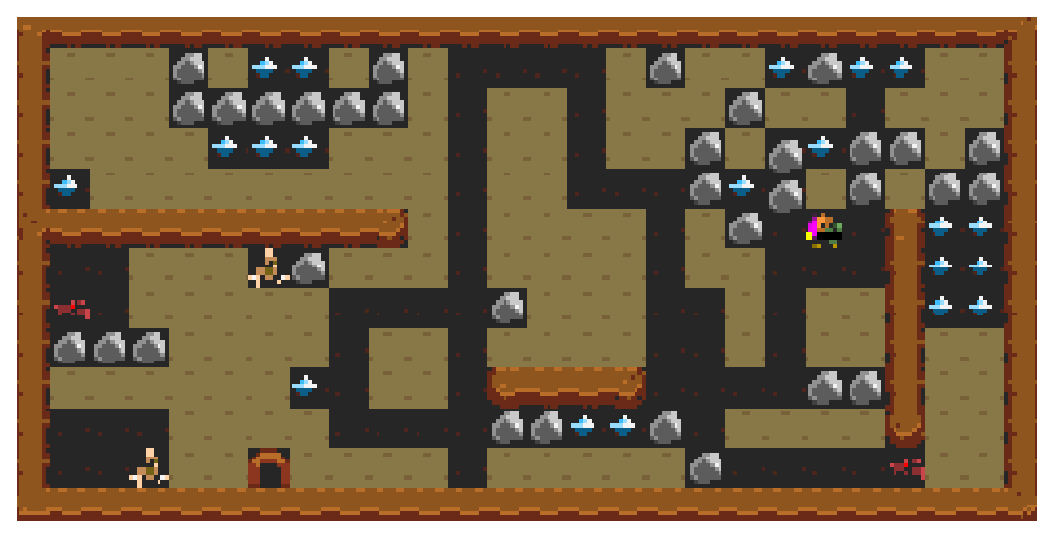
\includegraphics[width=0.48\textwidth]{./fig/gvgai-boulderdash-lvl0-v0-frame25}
    \label{subfig:b-frame1}
  } 
  \subfigure
  {
    \includegraphics[width=0.48\textwidth]{./fig/gvgai-boulderdash-lvl0-v0-frame26}
    \label{subfig:b-frame2}
  }
  \caption{Exemplos de execução do jogo \textit{Boulder Dash}.}
  \label{fig:boulderdashframe}
\end{center}
\end{figure}

Por fim, o \textit{Missile Command} parece ser possível de se jogar simplesmente aproximando-se dos mísseis mais próximos e os atacando. Entretanto é necessário um tempo de reação hábil para conseguir defender todos os canhões a tempo. As recompensas totais de cada fase variam conforme o número de canhões e mísseis inimigos também mudam, gerando uma distribuição de recompensas não linear. Na primeira fase do jogo, por exemplo, há quatro bolas de fogo e três canhões, levando a um total de oito pontos de recompensa. No PPO1 o agente não parecia ser capaz de manter uma pontuação perfeita pois alguns erros levaram a cinco pontos. Entretanto, em ambos PPO2 e PPO3 (Tabela \ref{tab:allgames}), os agentes foram capazes de melhorar sua performance, atingindo pontuação máxima na primeira fase do jogo. Apesar da variedade de exemplos no conjunto de treinamento ter levado a uma melhor exploração do conjunto de ação-estado, assim como nos outros jogos, é possível observar na Figura \ref{subfig:missilecommand-r} que os agentes ficaram restritos a um conjunto de sequência de ações que levaram ao sucesso nos jogos de treinamento.

\begin{figure}[ht]
 \begin{center}
  \subfigure
  {
    \includegraphics[width=0.48\textwidth]{./fig/gvgai-missilecommand-lvl0-v0-frame12}
    \label{subfig:m-frame1}
  } 
  \subfigure
  {
    \includegraphics[width=0.48\textwidth]{./fig/gvgai-missilecommand-lvl0-v0-frame13}
    \label{subfig:m-frame2}
  }
  \caption{Exemplos de execução do jogo \textit{Missile Command}.}
  \label{fig:missilecommandframe}
\end{center}
\end{figure}

Na Figura \ref{fig:avaliacao} é possível observar o desempenho médio de cada agente treinado, ao longo das cinco fases dos três jogos, em comparação a um agente com política aleatória. Assim como no jogo \textit{Missile Command}, todos os agentes foram direcionados a uma melhor exploração do espaço de ações a medida que aumentava a variedade da amostragem do conjunto de treinamento, levando a um aumento de desempenho geral ao longo das cinco fases de cada jogo. No entanto, nas fases que não foram utilizadas para compor o conjunto de treinamento, o desempenho se manteve muito próximo do agente com política aleatória.

% \begin{figure}[ht]
%  \centering
%   
\includegraphics[width=0.3\textwidth]{./fig/legend}
% \end{figure}

\begin{figure}[hb]
 \begin{center}
 \subfigure
  {
    \centering
\includegraphics[width=0.49\textwidth]{./fig/legend}
  } 
  \subfigure[\textit{Aliens}]
  {
    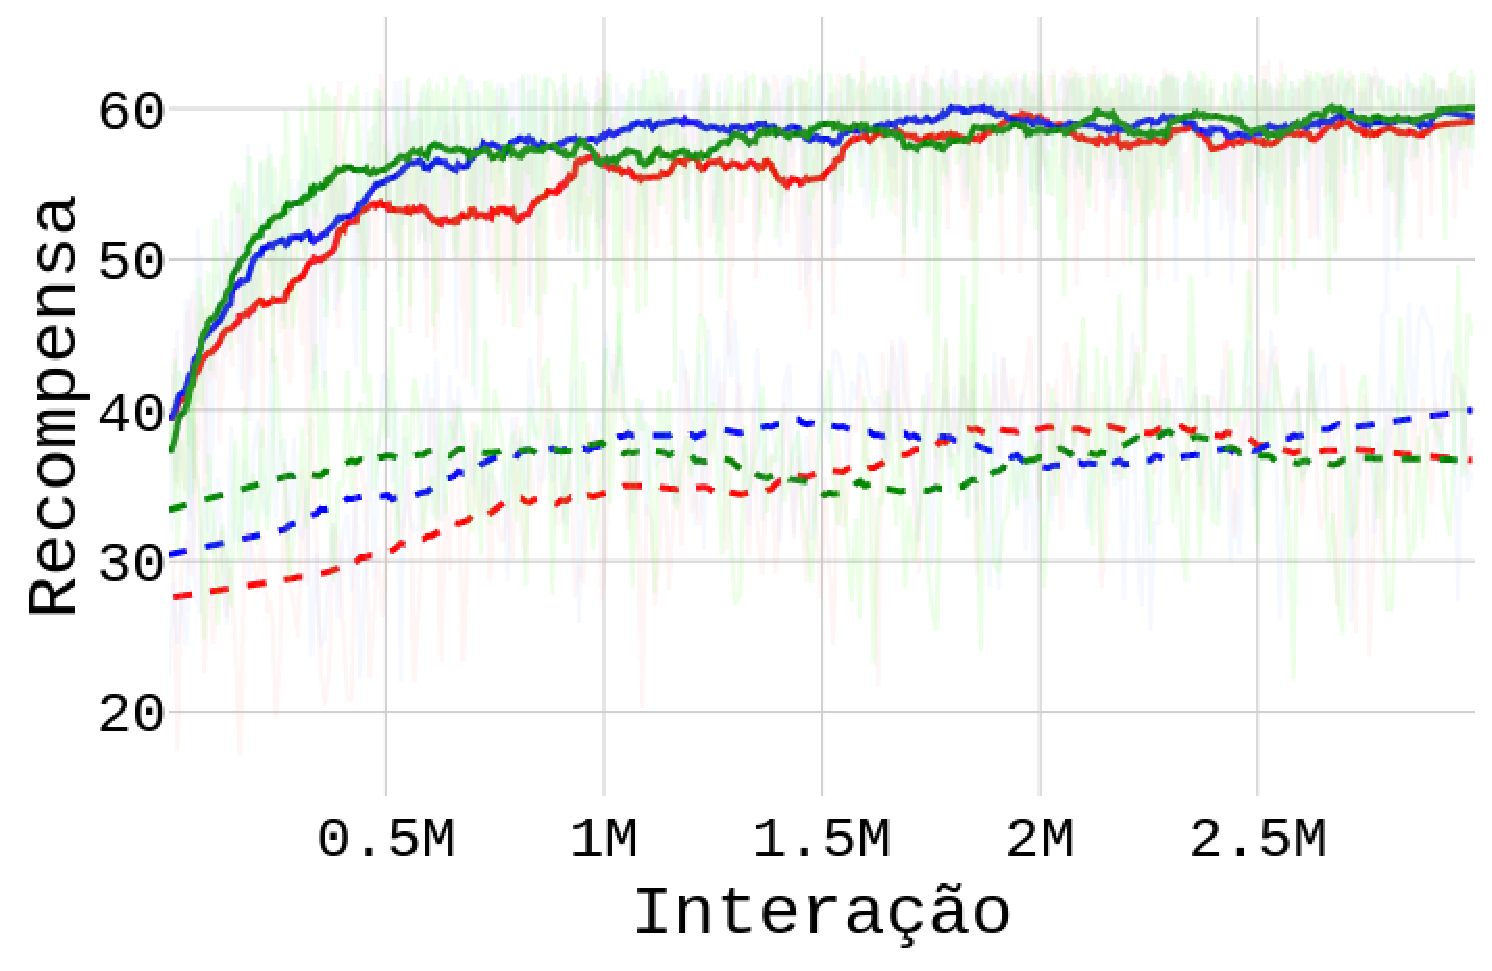
\includegraphics[width=0.48\textwidth]{./fig/aliens-results}
    \label{subfig:aliens-r}
  } 
  \subfigure[\textit{Boulder Dash}]
  {
    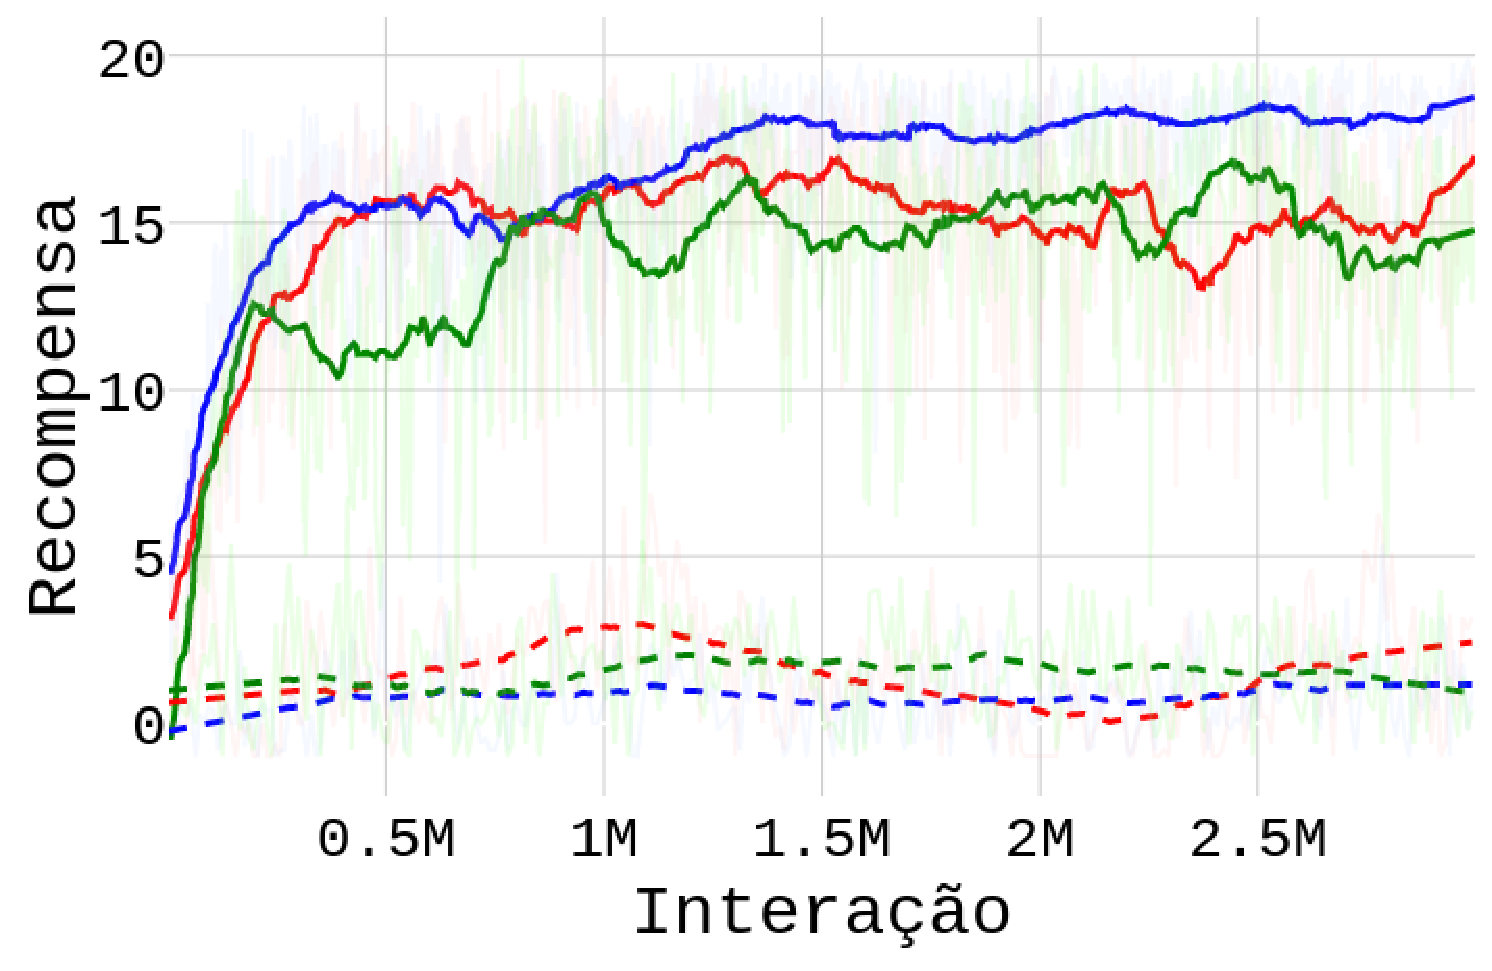
\includegraphics[width=0.48\textwidth]{./fig/boulderdash-results}
    \label{subfig:boulderdash-r}
  }
  \subfigure[\textit{Missile Command}]
  {
    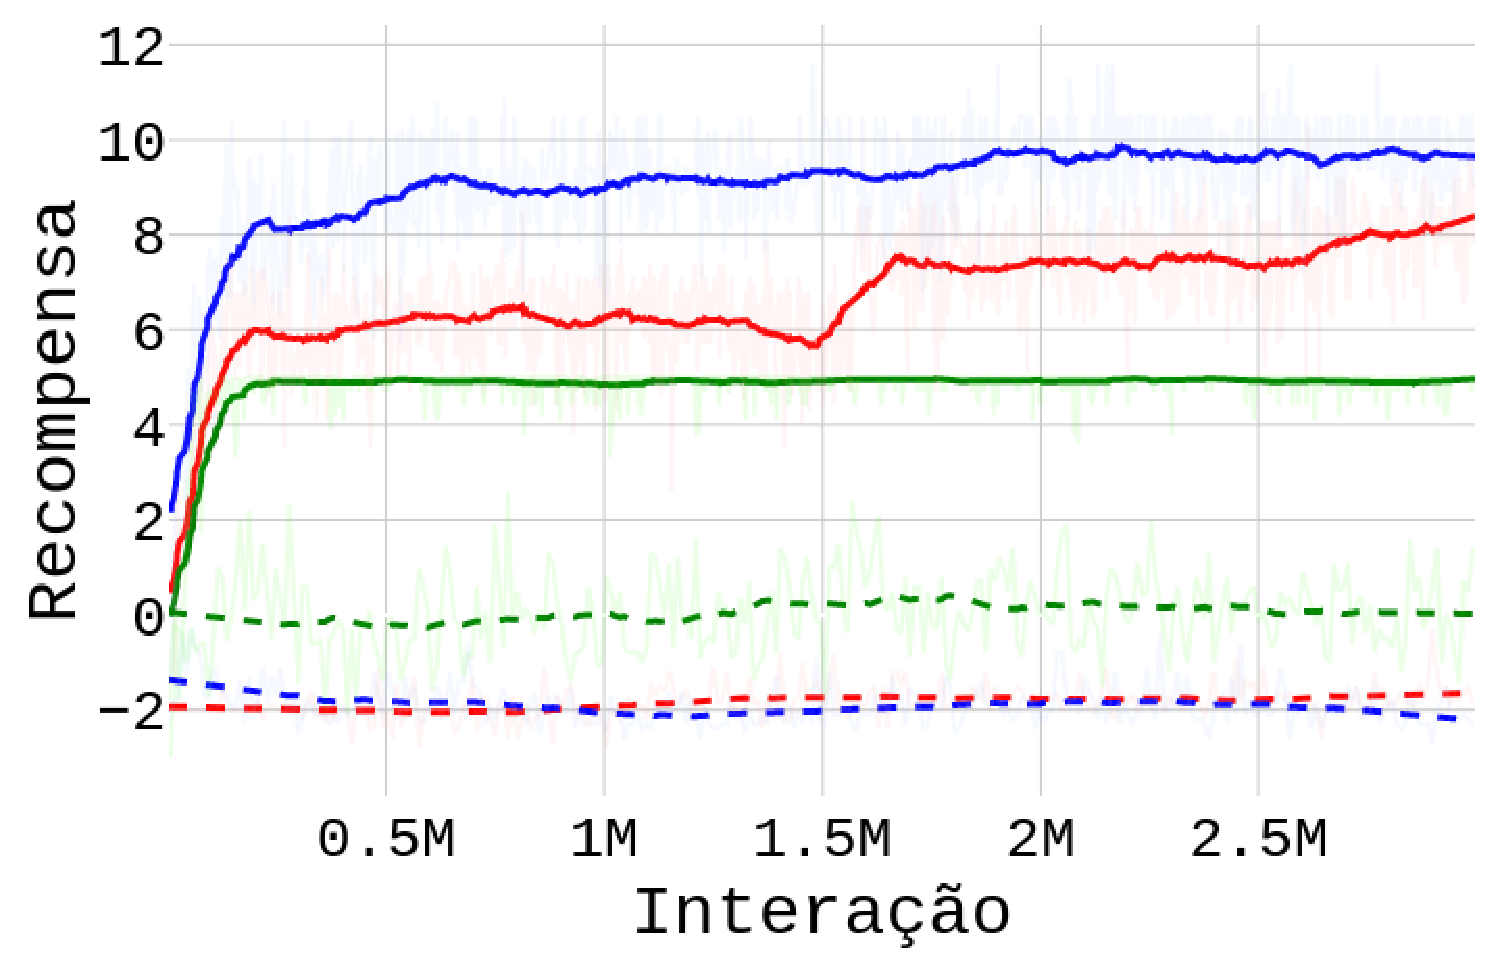
\includegraphics[width=0.48\textwidth]{./fig/missilecommand-results}
    \label{subfig:missilecommand-r}
  }
  \captionsetup{width=1\textwidth}
  \caption[Gráfico de relação treinamento-avaliação.]
  {Gráfico de relação treinamento-avaliação. Em vermelho, conjunto de treinamento com três fases (PPO3); em azul, conjunto de treinamento com duas fases (PPO2); em verde, conjunto de treinamento com uma fase (PPO1).}
  \label{fig:resultados}
\end{center}
\end{figure}
\begin{figure}[ht]
  \centering
  \subfigure[\textit{Aliens}]
  {
    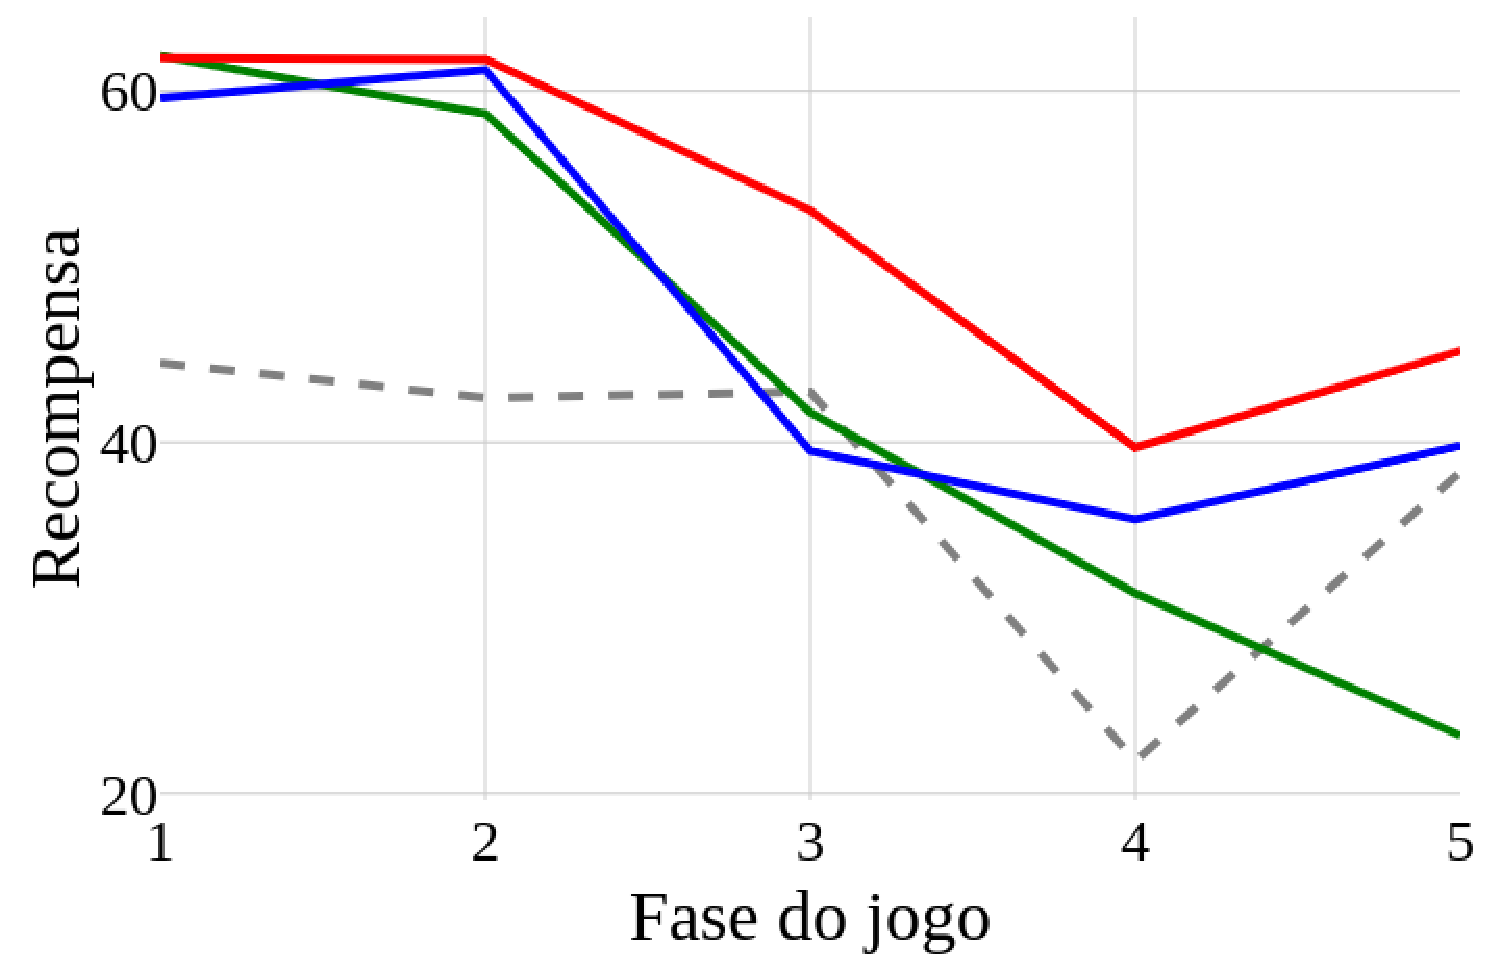
\includegraphics[width=0.45\textwidth]{./fig/aliens-evaluation}
    \label{subfig:aliens-a}
  } 
  \subfigure[\textit{Boulder Dash}]
  {
    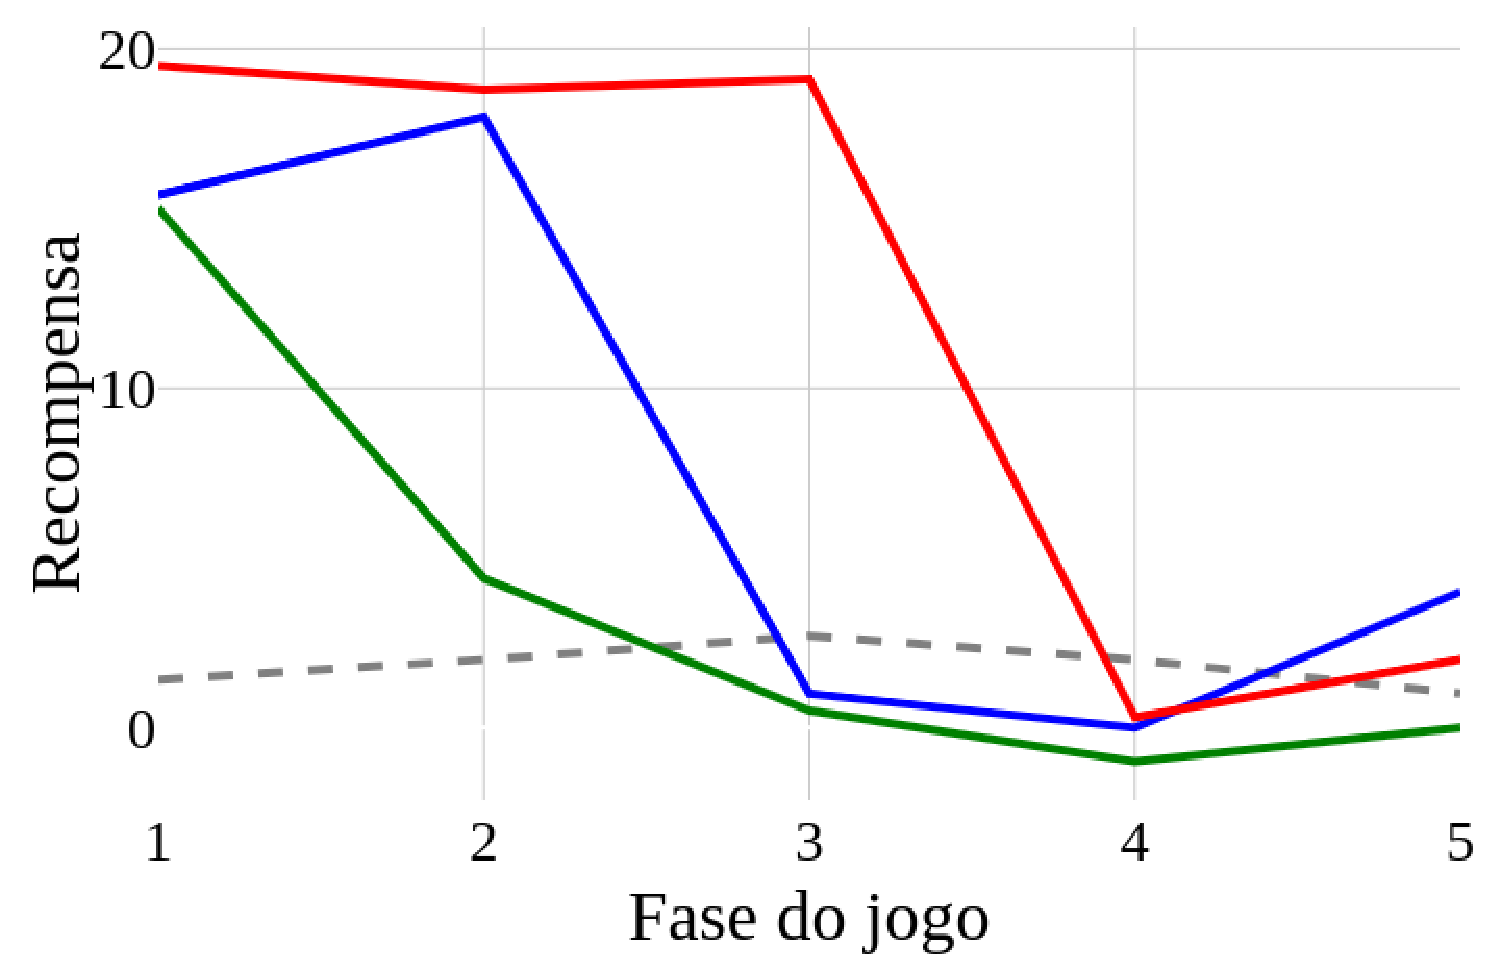
\includegraphics[width=0.45\textwidth]{./fig/boulderdash-evaluation}
    \label{subfig:boulderdash-a}
  }
  \subfigure[\textit{Missile Command}]
  {
    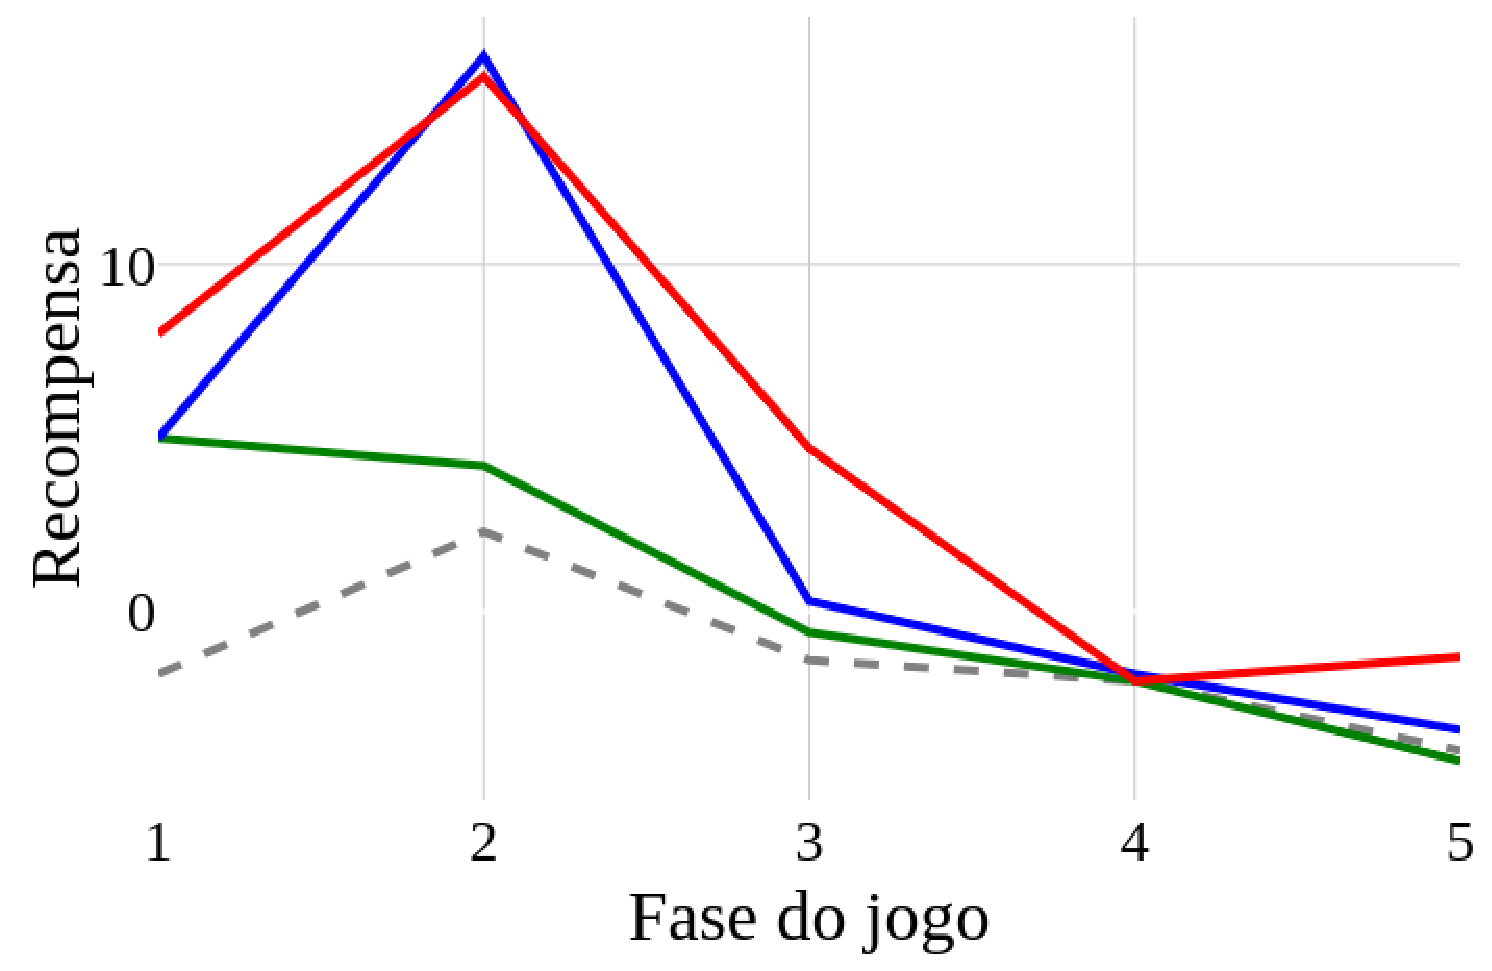
\includegraphics[width=0.45\textwidth]{./fig/missilecommand-evaluation}
    \label{subfig:missilecommand-a}
  }
  \captionsetup{width=1\textwidth}
  \caption[Gráfico de recompensa dos modelos treinados.]
  {Gráfico de recompensa dos modelos treinados. Em vermelho, conjunto de treinamento com três fases (PPO3); em azul, conjunto de treinamento com duas fases (PPO2); em verde, conjunto de treinamento com uma fase (PPO1); em linhas tracejadas, agente com política aleatória. }
  \label{fig:avaliacao}
\end{figure}